\parindent=0em
\section{Resumen y problemas de ARCore en Unity}
\noindent

Pese a la publicidad de ARCore y de su tecnología, una vez comprobada esta se puede asegurar que las opciones que ofrecen están todavía muy lejos del efecto deseado y que contienen varios problemas fundamentales.\\

En varias de las imágenes mostradas por la empresa se puede apreciar como se realiza una perfecta oclusión de los objetos virtuales junto a los objetos del mundo real, incluso generando mapas de calor para conocer con total seguridad la profundidad de la escena ~\ref{fig:ARDepth}. \\

Sin embargo, tras probar toda la tecnología, sabemos que los \textit{features} mencionados en capítulos anteriores se centran en encontrar los bordes de los objetos reales para generar la nube de puntos. Pese a ello, para crear los mapas de calor o una nube de puntos óptima también sería necesario que dichas \textit{features} se generasen en superficies planas.\\

\begin{figure}[H]
    \centering
    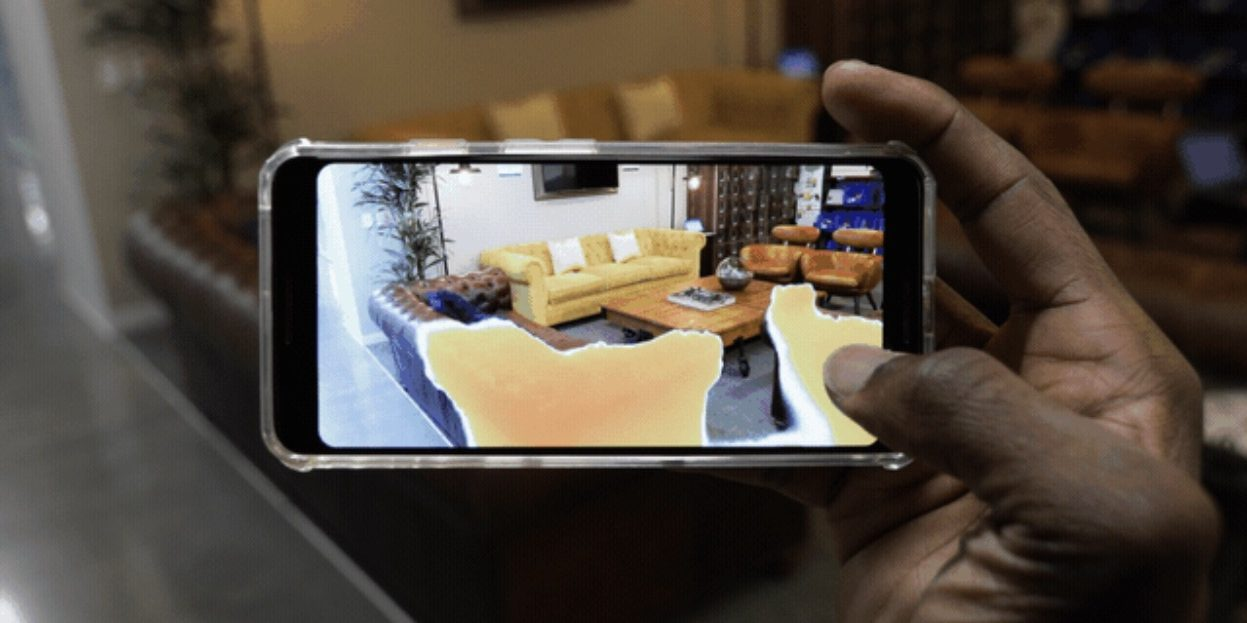
\includegraphics[scale=0.5]{Images/Optimización y resumen/ARDepth.jpg}
    \caption[Supuesto mapa de calor generado con ARCore.]{Supuesto mapa de calor generado con ARCore.}
    \label{fig:ARDepth}
\end{figure}

Pese a conocer que esta nube de puntos se genera principalmente con las \textit{features} en el contorno de los objetos, si se aumenta considerablemente el número de puntos que se pueden generar por cada frame se consigue una mejor oclusión. Esto sin embargo lleva a una caída bastante considerable del rendimiento de la aplicación así como a un consumo desmesurado de la batería del dispositivo, y por consiguiente también aumenta su temperatura.\\

A día de hoy realizar una oclusión con un nivel de detalle como el mostrado en los ejemplos de ARCore, desde un dispositivo móvil, es prácticamente imposible. Nos encontramos totalmente limitados por la tecnología de los dispositivos actuales.\\

Pese a todo esto, ARCore si que ha dado un gran paso dentro de la generación de oclusión en tiempo real. Su tecnología no precisa tener varias cámaras integradas ni sensores ToF para realizar un escaneo de la profundidad. En el futuro, cuando toda la tecnología de dispositivos móviles mejore, se podrá realizar oclusión en tiempo real sin ningún problema, aunque de momento sólo servirá para realizar fotogrametría de manera asíncrona.\\